% MATH 5131 - Introduction to Mathematical Methods and Modeling - Assignment 1

\documentclass{article}
\usepackage[utf8]{inputenc}
\usepackage[english]{babel}
\usepackage[]{amsthm}
\usepackage[]{amsmath,amssymb}
\usepackage[table]{xcolor}
\usepackage{blindtext}
\usepackage{multicol}
\usepackage{color}
\usepackage{comment}
\usepackage{wrapfig}
\usepackage{graphicx}
\usepackage{listings}
\usepackage{xcolor}
\usepackage{float}
\usepackage[a4paper, total={6in, 8in}]{geometry}
\setlength{\columnseprule}{1pt}
\def\columnseprulecolor{\color{gray}}

\definecolor{codegreen}{rgb}{0,0.6,0}
\definecolor{codegray}{rgb}{0.5,0.5,0.5}
\definecolor{codepurple}{rgb}{0.58,0,0.82}
\definecolor{backcolour}{rgb}{0.95,0.95,0.92}

\lstdefinestyle{codestyle}{
	backgroundcolor=\color{backcolour},   commentstyle=\color{codegreen},
	keywordstyle=\color{magenta},
	numberstyle=\tiny\color{codegray},
	stringstyle=\color{codepurple},
	basicstyle=\ttfamily\footnotesize,
	breakatwhitespace=false,         
	breaklines=true,                 
	captionpos=b,                    
	keepspaces=true,                 
	numbers=left,                    
	numbersep=5pt,                  
	showspaces=false,                
	showstringspaces=false,
	showtabs=false,                  
	tabsize=2
}

\lstset{style=codestyle}

\usepackage{graphicx}
\graphicspath{ {./images/} }

\usepackage[rightcaption]{sidecap}
\usepackage{wrapfig}

\setlength{\arrayrulewidth}{1mm}
\setlength{\tabcolsep}{18pt}
\renewcommand{\arraystretch}{1.2}

\title{Assigment 1 - Solutions}
\author{Sai Nikhil}
\date\today


\newenvironment{solution}
{\renewcommand\qedsymbol{$\blacksquare$}\begin{proof}[Solution]}{\end{proof}}


\begin{document}
\maketitle

\subsection*{Problem 1}
Find the general solution to \[ t \frac{dy}{dt} - 2ty = t^2 - t \]
\begin{solution}
	The given equation holds true when,
\[ t = 0 \quad or \quad \frac{dy}{dt} - 2y = t - 1 \] \\
The integration factor for the above differential equation = $ e^{\int -2dt} $ = $ e^{-2t} $ \\ \\
Therefore the solution is given by,
\begin{equation}
\begin{split}
y(t) & = e^{2t}\int{e^{-2t}(t - 1)dt}\\
& = e^{2t} \left(\frac{te^{-2t}}{-2} - \int{\frac{e^{-2t}}{-2}} - \frac{e^{-2t}}{-2} + c_1\right) \\
& = e^{2t} \left(-\frac{te^{-2t}}{2} - \frac{e^{-2t}}{4} + \frac{e^{-2t}}{2} + c\right) \\
& = -\frac{t}{2} + \frac{1}{4} + ce^{2t}
\end{split}
\end{equation}


\end{solution}


\subsection*{Problem 2}
Draw the slope plot for $\frac{dy}{dt} = (1-t)y$ and the trajectory $y(0) = 0$.
\begin{solution}
	The following table represents values of $\frac{dy}{dt}$ for first few values of $y$ and $t$.
	
	\begin{center}
		{\rowcolors{3}{gray!30}{white}
			\begin{tabular}{ |p{3cm}|p{3cm}|p{3cm}| }
				\hline
				\multicolumn{3}{|c|}{Slope plot} \\
				\hline
				\multicolumn{1}{|c|}{$t$} & \multicolumn{1}{c|}{$y$} & \multicolumn{1}{c|}{$\frac{dy}{dt} = (1-t)y $} \\
				\hline
				\multicolumn{1}{|c|}{0} & \multicolumn{1}{c|}{0} & \multicolumn{1}{c|}{0} \\
				\multicolumn{1}{|c|}{0} & \multicolumn{1}{c|}{1} & \multicolumn{1}{c|}{1} \\
				\multicolumn{1}{|c|}{1} & \multicolumn{1}{c|}{0} & \multicolumn{1}{c|}{0} \\
				\multicolumn{1}{|c|}{1} & \multicolumn{1}{c|}{1} & \multicolumn{1}{c|}{0} \\
				\multicolumn{1}{|c|}{0} & \multicolumn{1}{c|}{-1} & \multicolumn{1}{c|}{-1} \\
				\multicolumn{1}{|c|}{-1} & \multicolumn{1}{c|}{0} & \multicolumn{1}{c|}{0} \\
				\multicolumn{1}{|c|}{-1} & \multicolumn{1}{c|}{1} & \multicolumn{1}{c|}{2} \\
				\multicolumn{1}{|c|}{1} & \multicolumn{1}{c|}{-1} & \multicolumn{1}{c|}{0} \\
				\multicolumn{1}{|c|}{-1} & \multicolumn{1}{c|}{-1} & \multicolumn{1}{c|}{-2} \\
				\hline
			\end{tabular}
		}
\newline
\newline
\newline

	\end{center}


Following is the Python code to draw the slope plot using matplotlib library:

\begin{lstlisting}[language=Python, caption=Slope plot code]

import numpy as np
from matplotlib import pyplot as plt

def diff(t,y):
    return (1-t)*y

t = np.linspace(-4,4,20)
y = np.linspace(-4,4,20)

for j in t:
    for k in y:
        slope = diff(j,k)
        domain = np.linspace(j-0.05,j+0.05,2)
        def fun(t1,y1):
            z = slope*(domain-t1)+y1
            return z
        plt.plot(domain,fun(j,k),solid_capstyle='projecting',solid_joinstyle='bevel')
        
plt.rcParams["figure.figsize"] = (10,10)
plt.grid(True)
plt.show()
\end{lstlisting}
\begin{figure}[H]
\caption{Slope plot for $\frac{dy}{dt} = (1-t)y$}
\centering
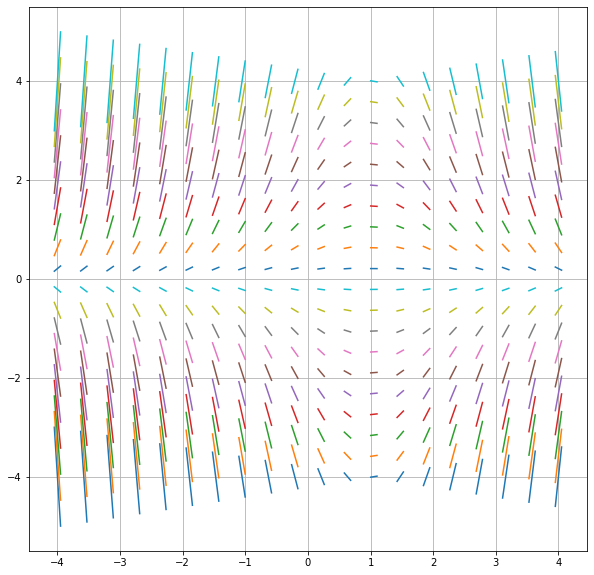
\includegraphics[width=1.0\textwidth]{slope_plot}
\end{figure}
Solving the initial value problem,
	$\frac{dy}{dt} = (1-t)y \quad y(0) = 0$
we get, \\
\begin{equation}
\begin{split}
	\frac{dy}{y} & = (1-t)dt\\
\end{split}
\end{equation}
Integrating on both sides,
\begin{equation}
\begin{split}
	\int{\frac{dy}{y}} &= \int{(1-t)dt}\\
	ln(y) &= t-\frac{t^2}{2}+c_1\\
	y(t) &= ce^{t-\frac{t^2}{2}}\\
\end{split}
\end{equation}
Substituting the initial conditions, we get,
\begin{equation}
\begin{split}
	y(t) = 0
\end{split}
\end{equation}

\begin{figure}[H]
\caption{Solution to I.V.P. $\frac{dy}{dt} = (1-t)y \quad y(0) = 0$}
\centering
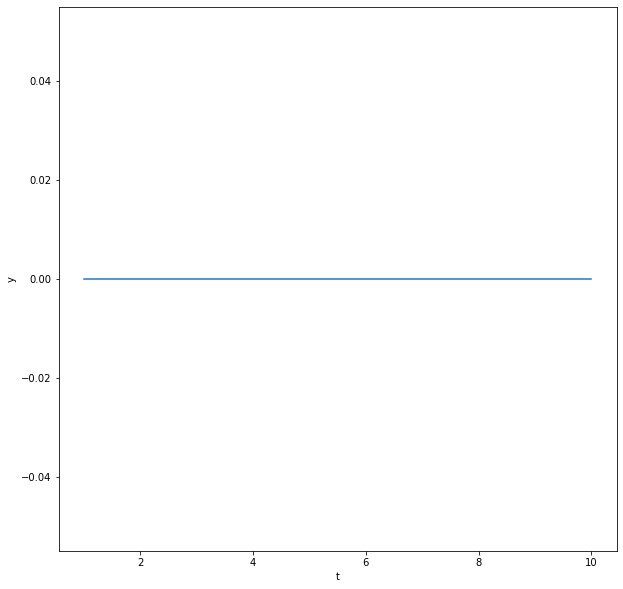
\includegraphics[width=1.0\textwidth]{solution}
\end{figure}

\end{solution}


\subsection*{Problem 3}
Consider the lake system with Lake A flowing into Lake B. Lake A is contaminated with arsenic
due to a coal gasification plant out-flowing near the lake. Clean water enters Lake A at a rate $F$
and all water flows into Lake B. Write a pair of differential equations, one for the concentration of
pollutants in Lake A and one for Lake B. Solve the system of differential equations by first solving
for Lake A and then for Lake B.
\begin{solution}
Given, rate of inflow into Lake A = $F \; lit/min$ \\
Let us assume,
\begin{enumerate}
	\item The volumes of Lake A, Lake B be $V_1$ and $V_2$ ($V_1 \ne V_2$) respectively.
	\item The amount of Arsenic at a time $t$ in Lake A, Lake B be $P_1(t)$ and $P_2(t)$ respectively.
	\item The initial amount of Arsenic in Lake A be $P_1(t=0) = P_0$
	\item The initial amount of Arsenic in Lake B be $0$.
\end{enumerate}
Applying compartment model for two lakes with the above information, we get,

\begin{multicols}{2}

\begin{figure}[H]
\caption{Compartment Model for Lake A}
\centering
\includegraphics[width=0.5\textwidth]{"Problem3 - Left Compartment"}
\end{figure}
\vspace*{\fill}
\begin{equation}
\begin{split}
\frac{dP_1(t)}{dt} &= 0 - \frac{F \times P_1(t)}{V_1}\\
\frac{dP_1(t)}{dt} &= -\frac{FP_1}{V_1}\\
P_1(t) &= P_0e^{-\frac{Ft}{V_1}}\\
\end{split}
\end{equation}
\vspace*{\fill}

\columnbreak

\begin{figure}[H]
\caption{Compartment Model for Lake B}
\centering
\includegraphics[width=0.5\textwidth]{"Problem3 - Right Compartment"}
\end{figure}

\begin{equation}
\begin{split}
&\frac{dP_2(t)}{dt} = \frac{F \times P_1(t)}{V_1} - \frac{F \times P_2(t)}{V_2}\\
&\frac{dP_2}{dt} + \frac{FP_2}{V_2} = \frac{FP_1}{V_1}\\
\end{split}
\end{equation}

Substituting equation (5) into (6), we get,

\begin{equation}
\begin{split}
\frac{dP_2}{dt} + \frac{FP_2}{V_2} &= \frac{FP_0}{V_1}e^{-\frac{Ft}{V_1}}\\
\end{split}
\end{equation}
Using, integrating factor (I.F.) = $e^{\int{\frac{F}{V_2}dt}}$ = $e^{\frac{Ft}{V_2}}$\\
And initial condition $P_2(0) = 0$\\
The solution is,
\begin{equation}
\begin{split}
P_2(t) &= e^{\frac{-Ft}{V_2}}\int{e^{\frac{Ft}{V_2}}\left(\frac{F}{V_1}P_0e^{\frac{-Ft}{V_1}}\right)}dt\\
P_2(t) &= \frac{P_0V_2}{V_2-V_1}\left(e^{\frac{-Ft}{V_2}} - e^{\frac{-Ft}{V_1}}\right)
\end{split}
\end{equation}


\end{multicols}


\end{solution}


\subsection*{Problem 4}
A bar opens at $6 \; PM$ and allows smoking. Smoke contains $4\%$ carbon monoxide and enters the
room at a constant rate of $.006 \; m^3/min$. Given that the bar's floor area is $20 m$ by $15 m$ by $4
m$ and the bar's ventilation system removes the smoke-air mixture at a $10$ times the rate smoke is
produced, set up a initial value problem for the concentration of smoke in the bar.
Prolonged expose to a concentration of more than $0.012\%$ carbon monoxide can be fatal. At
what time will the lethal limit be reached?

\begin{solution}
Given,
\begin{enumerate}
\item inflow of carbon monoxide, $F_{in} = .006 \; m^3/min$.
\item outflow of carbon monoxide, $F_{out}$ = $10 \times F_{in} = .06 \; m^3/min$.
\item volume of bar, $V$ = $20 \times 15 \times 4 \; m^3 = 1200 \; m^3$.
\item input concentration of carbon monoxide into bar, $C_{in} = 4\%$.
\item intial concentration of carbon monoxide in the bar, $C(0) = 0$.
\end{enumerate}
Let us assume,\\
Concentration of carbon monoxide in bar at time $t = C(t) = C$\\
Applying compartment model for the bar with the above information, we get,\\

\begin{figure}[H]
\caption{Compartment Model for bar}
\centering
\includegraphics[width=1.0\textwidth]{"Problem 4"}
\end{figure}

\begin{equation}
\begin{split}
\frac{dC}{dt} = \frac{F_{in}}{V}C_{in}-\frac{F_{out}}{V}C_{out}
\end{split}
\end{equation}
The solution to the above equation is,
\begin{equation}
\begin{split}
C(t) = \frac{F_{in}C_{in}}{F_{out}}\left(1-e^{-\frac{F_{out}}{V}t}\right)
\end{split}
\end{equation}
The lethal limit for carbon monoxide is $0.012\%$. Let, $t_h$ be the time when lethal limit is reached.\\
Therefore, $C(t_h) = 0.012\%$.\\
Substiting this in equation (10), we get,\\
\begin{equation}
\begin{split}
0.012 &= \frac{0.006 \times 4}{0.06}\left(1-e^{-\frac{0.06}{1200}t_h}\right)\\
\implies t_h &= 609.184 \; min. \\
&\approx \boxed{10 \; hr.}
\end{split}
\end{equation}



\end{solution}


\end{document}